
\subsection{准确解}
$u(x, t) = e^{-at}f(x + t)$


\subsection{Leap-Frog}
$h = 2\pi / 2^p, p \in [5, 13], k = h / 2, T = 2\pi / 10$,

对于初值$f = \sin x + \sin (10 * x),
  f = \sin x + \sin (100 * x)$ 数值计算误差如下表和图.
\begin{table}[!h]
  \resizebox{.8\textwidth}{!}{%
    \begin{tabular}{|c|c|c|c|c|c|c|c|c|c|}
      \hline
      h      & 1/32 & 1/64                 & 1/128                & 1/256                & 1/512                & 1/1024               & 1/2048               & 1/5096               & 1/10192              \\ \hline
      error1 & 0.74 & 0.45                 & 0.15                 & $4.4 \times 10^{-2}$ & $2.3 \times 10^{-2}$ & $1.4 \times 10^{-2}$ & $5.6 \times 10^{-3}$ & $1.9 \times 10^{-3}$ & $9.3 \times 10^{-4}$ \\ \hline
      error2 & 0.68 & 0.67                 & 0.12                 & 0.68                 & 0.15                 & 0.75
             & 0.31 & $7.7 \times 10^{-2}$ & $2.2 \times 10^{-2}$                                                                                                                                           \\ \hline
    \end{tabular}%
  }
  \centering
  \caption{两种初值情况下计算到$t_n = 2\pi / 10$时的
    L2误差}
  \label{tab:my-table}
\end{table}

\begin{figure}[!h]
  \centering
  \subfigure[$error$]{
    \begin{minipage}[t]{0.5\linewidth}
      \centering
      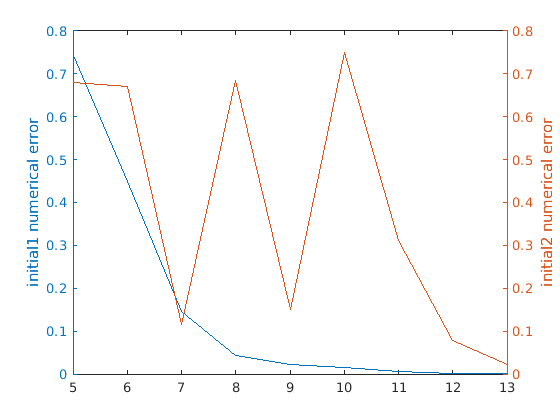
\includegraphics[height=2.5in, width=2.5in]{fig/error.png}
      %\caption{fig1}
    \end{minipage}%
  }%
  \subfigure[$log(error)$]{
    \begin{minipage}[t]{0.5\linewidth}
      \centering
      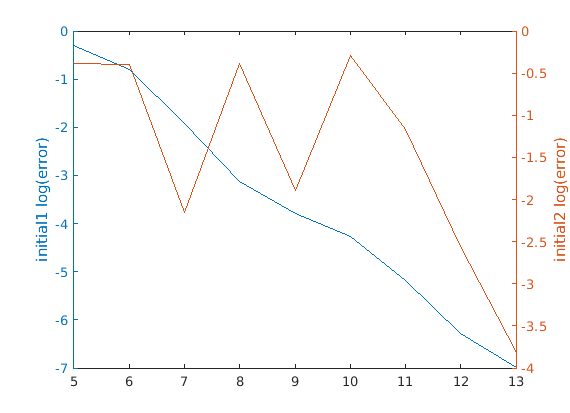
\includegraphics[height=2.5in, width=2.5in]{fig/logError.png}
      %\caption{fig2}
    \end{minipage}%
  }%
\end{figure}

由图表可发现, 收敛精度为一阶, 且当初值条件震动频率高
时需要更细的网格使得计算误差达到可接受范围,


\subsection{CFL condition}
取$k = 1.1h$不满足CFL condition计算数值结果, $h = 1/2048$
在两种初值条件下, $t_n = T$时的误差L2范数分别为$1.54 \times 10^{14},
  1.63 \times 10^{15}$ .
见LeapFrogPeriodTest1.m中计算结果CFLError1, CFLError2.
由explosion的误差可知不满足CFL condition时结果不会收敛.